\documentclass[conference]{IEEEtran}
\usepackage{blindtext, graphicx}
\usepackage{amsmath}
\usepackage{listings}


\ifCLASSINFOpdf
\else
\fi


% correct bad hyphenation here
\hyphenation{op-tical net-works semi-conduc-tor}


\begin{document}

\title{Chimera - Simple Agnostic Language Framework using Node.js and Command Line 
Arguments for Stand Alone and Distributed Computing}

\author{\IEEEauthorblockN{Go Frendi Gunawan}
\IEEEauthorblockA{STIKI Malang\\ Malang, Indonesia\\
Email: frendi@stiki.ac.id}
\and
\IEEEauthorblockN{Mukhlis Amien}
\IEEEauthorblockA{STIKI Malang\\
Malang, Indonesia\\
Email: amien@stiki.ac.id}
\and
\IEEEauthorblockN{Jozua Ferjanus Palandi}
\IEEEauthorblockA{STIKI Malang\\
Malang, Indonesia\\
Email: jozuafp@stiki.ac.id}}

% make the title area
\maketitle


\begin{abstract}
%\boldmath
Component Based Software Engineering (CBSE) is a branch of software 
engineering that emphasizes the separation of concerns with respect to the 
wide-ranging functionality available throughout a given software system.  The 
main advantage of CBSE is separation of components. A single component will 
only focus on a single task or related collection of tasks. Allowing software 
developer to reuse the component for other use-cases. By using this approach, 
software developer doesn't need to deal with spaghetti code. Several 
approaches has been developed in order to achieve ideal CBSE. The earliest 
implementation was UNIX pipe and redirect, while the newer approach including 
CORBA, XML-RPC, and REST. Our framework, Chimera, was built on top of Node.js. 
Chimera allows developer to build pipe flow in a chain (a YAML formatted file) 
as well as defining global variables. Compared to UNIX named and unnamed pipe, 
this format is easier and more flexible. On the other hand, unlike XML-RPC, 
REST, and CORBA, chimera doesn't enforce users to use special protocol such as 
HTTP (except for distributed computing scenario). Nor it require the components
to be aware that they works on top of the framework.
\end{abstract}

% Note that keywords are not normally used for peerreview papers.
\begin{IEEEkeywords}
Chimera, Language Agnostic, Component-Based Software Engineering, CBSE, Node.js, CLI.
\end{IEEEkeywords}

\IEEEpeerreviewmaketitle

\section{Introduction}

Component based software development approach is based on the idea to develop 
software systems by selecting appropriate off-the shelf components and then to 
assemble them with a well-defined software architecture \cite{kaur2010component}.

In order to implement component-based software engineering (CBSE), several 
approaches has beeen performed. The earliest attempt was UNIX pipe mechanism 
\cite{mcilroy1968mass}. Pipe mechanism was not the only attempt to achieve CBSE.
The more modern approaches including XML-RPC \cite{xmlrpc} and JSON-RPC \cite{jsonrpc}. 
Later, Object Management Group (OMG) introduced a new standard named CORBA (Common
Object Request Broker Architecture) \cite{corba}. Another interesting approach was 
introduced by Two Sigma Open Source. Two Sigma created a platform known as Beaker
Notebook \cite{beakernotebook}. Beaker Notebook is mainly used for research purpose. 
On 2016, Feilhauer and Sobotka introduce another platform called DEF 
\cite{feilhauer2016def}.

Aside from Unix Pipe, all other mechanism require the components to be aware that 
they are part of the framework. This means that you cannot use old programs (e.g:
{\it cal} and {\it cowsay}) as XML-RPC or CORBA component. At least additional layer
and adjustment has to be built.

CORBA, XML-RPC, SOAP, and JSON-RPC also needs HTTP protocol since they were designed for 
in client-server architecture. It imply that developers need to build a web server in 
order to use the mechanisms. However, in any use case that only need a single computer,
this is not ideal.

Considering the advantages and disadvantages of earlier approaches, in this paper, 
we develop a new CBSE framework named Chimera. This framework is much simpler since
HTTP is only required for distributed computation. Chimera also use CLI mechanism that
works in almost all OS and most programming language.
The only dependency of Chimera are Node.js and several NPM packages.

\section{Previous Research}

In this section we will have an indepth discussion about previous CBSE implementation 
preceeding Chimera.


\subsection{UNIX Pipe}

The very first implementation of CBSE was UNIX pipe mechanism \cite{mcilroy1968mass}. 
UNIX pipe allows engineer to pass output of a single program as an input of 
another program. Since a lot of server is UNIX or linux based, this pipe 
mehanism availability is very high. Even DOS also provide similar mechanism 
\cite{dos7command}.

Pipe mechanism works by letting a program's standard output being used as another
program's standard input. By putting several programs into a single pipeline, we can
compose a more complex process as shown in figure ~\ref{fig:unixPipe}.

\begin{figure}
	\centering
	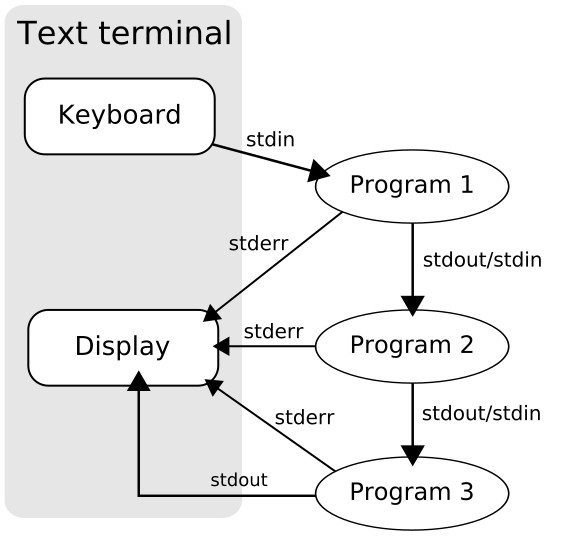
\includegraphics[width=0.3\textwidth]
		{images/Pipeline.jpg}
	\caption{Unix Pipeline Mechanism}
	\label{fig:unixPipe}
\end{figure}

For more explanation, we provide a simple test case. Consider two different program,
{\it cal} and {\it cowsay}. Given no argument, {\it cal} will show you current month's
calendar. On the other hand, given a single argument, {\it cowsay} will show the 
argument alongside an ASCII art of a cow.

\begin{lstlisting}[caption=cal and cowsay, label=calAndCowsay, language=bash, basicstyle=\small, breaklines=true]
#! cal
     June 2017        
Su Mo Tu We Th Fr Sa  
             1  2  3  
 4  5  6  7  8  9 10  
11 12 13 14 15 16 17  
18 19 20 21 22 23 24  
25 26 27 28 29 30     
                      
#! cowsay "hello"
 _______
< hello >
 -------
        \   ^__^
         \  (oo)\_______
            (__)\       )\/\
                ||----w |
                ||     ||
\end{lstlisting}

Unix pipe mechanism allows you to combine those two programs. For example, if you
want the output of {\it cal} become the input of {\it cowsay}, you can use pipe
command as shown in listing ~\ref{unnamedPipeExample}

\begin{lstlisting}[caption=Unnamed pipe example, label=unnamedPipeExample, language=bash, basicstyle=\small, breaklines=true]
#! cal | cowsay
 ________________________________________
/  June 2017 Su Mo Tu We Th Fr Sa        \
|                                        |
| 1 2 3                                  |
|                                        |
| 4 5 6 7 8 9 10 11 12 13 14 15 16 17 18 |
\ 19 20 21 22 23 24 25 26 27 28 29 30    /
 ----------------------------------------
        \   ^__^
         \  (oo)\_______
            (__)\       )\/\
                ||----w |
                ||     ||
\end{lstlisting}


Beside of it's high availability and simplicity, UNIX pipe also support parallel
processing through named-pipe mechanism. The named-pipe mechanism can be used to 
provide cheap parallel processing \cite{conway2003parallel}. 

In listing ~\ref{namedPipeExample} we show a simple named-pipe mechanism. First, we make
a named pipe called {\it backpipe} by using {\it mkfifo} command. Next, we redirect
standard output of {\it cal} and {\it cowsay} into {\it backpipe}. Finally, we show
the content of the {\it backpipe} by using {\it cat} command.

\begin{lstlisting}[caption=Named pipe example, label=namedPipeExample, language=bash, basicstyle=\small, breaklines=true]
#! mkfifo backpipe 

#! cal > backpipe | cowsay hello > backpipe | cat backpipe
     June 2017        
Su Mo Tu We Th Fr Sa  
             1  2  3  
 4  5  6  7  8  9 10  
11 12 13 14 15 16 17  
18 19 20 21 22 23 24  
25 26 27 28 29 30     
                     
 _______
< hello >
 -------
        \   ^__^
         \  (oo)\_______
            (__)\       )\/\
                ||----w |
                ||     ||
\end{lstlisting}

Although pipe mechanism provide high availability and capability, 
it has several limitations. For example, named-pipe needs external file as temporary 
container. The external file has to be deleted once the operation performed. 
This approach is not straight forward, thus, some efforts is needed in order to 
to build a working named-pipe based computation. 

For simple use cases involving a single computer, pipe mechanisme might be ideal. 
However, at some point, when the program become more complicated, memory sharing 
and network access might be needed. Using a mere pipe mechanism to support those 
requirement is either hard or impossible.

\subsection{CORBA}

From CORBA official website, CORBA is defined as standard created by the Object 
Management Group designed to facilitate the communication of systems 
that are deployed on diverse platforms \cite{corba}. CORBA 1.0 was released on August 
1991. The last version, CORBA 3.3 was released on November 2012 \cite{corbaspec}.
CORBA is heavily affected by object oriented paradigm.

The main component of CORBA is the Object Request Broker (ORB). ORB act as bridge 
between client and service provider. The service provider (server) provide an 
implementation of an object. While the client can be a user interface that depend on
the service provided by the server. Both, client and server needs to agree about the
object structure. This agreement is written in an Interface Description Language (IDL).
The IDL in server side is called skeleton, while the IDL in client side is called stub.

\begin{figure}
	\centering
	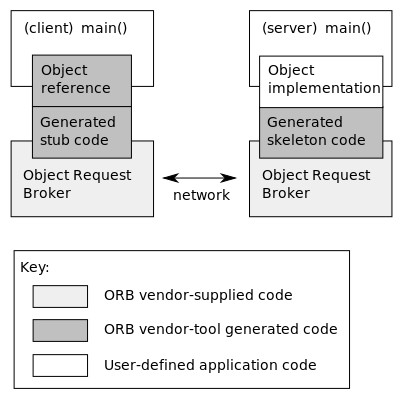
\includegraphics[width=0.3\textwidth]
		{images/Orb.jpg}
	\caption{Object Request Broker}
	\label{fig:orb}
\end{figure}

Figure ~\ref{fig:orb} shows the interaction between ORB, server, and client.
IDL can be written in Java, C++, or any other language, depend on the implementation of
the ORB.

An IDL example is shown in listing ~\ref{corbaIDLExample}.

\begin{lstlisting}[caption=CORBA IDL Example in C++, label=corbaIDLExample, language=c, basicstyle=\small, breaklines=true]
module Finance {
  typedef sequence<string> StringSeq;
  struct AccountDetails {
    string     name;
    StringSeq  address;
    long       account_number;
    double     current_balance;
  };
  exception insufficientFunds { };
  interface Account {
    void deposit(in double amount);
    void withdraw(in double amount) raises(insufficientFunds);
    readonly attribute AccountDetails details;
  };
};
\end{lstlisting}

Compared to UNIX Pipe, CORBA is more feature rich and complex. The developer needs to 
embrace OOP paradigm as well as being familiar with IDL and the CORBA architecture. 
Despite of it's language agnoticism, some non OOP language (e.g: Matlab and GNU Octave) 
is not supported by CORBA \cite{feilhauer2016def}. CORBA also suffer of several 
criticism \cite{henning2006rise}. Even OOP as the foundation of CORBA, also face several 
critics \cite{hadar2013intuition} regardless of it's popularity.


\subsection{XML-RPC, SOAP, and JSON-RPC}

XML-RPC is a spec and a set of implementations that allow software running on 
disparate operating systems, running in different environments to make procedure 
calls over the Internet. XML-RPC using HTTP as the transport and XML as the encoding. It is designed to be as simple as possible, while allowing complex data structures to be transmitted, processed and returned \cite{xmlrpc}.

SOAP stands for Simple Object Access Protocol. SOAP is a lightweight protocol 
intended for exchanging structured information in a decentralized, distributed 
environment \cite{soap}. SOAP was built on top of XML-RPC. It uses XML format as 
well as HTTP protocol.

JSON-RPC is lightweight remote procedure call protocol similar to XML-RPC 
\cite{jsonrpc}. The main difference between XML-RPC and JSON-RPC is the data transfer
format. In most cases, JSON is more lightweight compared to XML.

XML-RPC, SOAP, and JSON-RPC are heavily depend on HTTP for inter-process-communication 
protocol. This is ideal for client-server architecture as HTTP is quite common and
easy to be implemented.

Those three methods are basically another implementation of RPC (Remote Procedure Call). 
Compared to CORBA, these three methods are more flexible. With the exception of SOAP,
they don't enforce developer to embrace OOP paradigm.

In terms of language agnoticism, XML-RPC and JSON-RPC support any language that can
access HTTP and parse/create the data format. However, in order to use these protocols,
a developer should be aware that the components they built will works as a part of the
bigger system. Tools or programs that were built without this consideration will need
some adjustment or additional layers in order to make them works with the protocol.
For example, using {\it{cowsay}} or {\it{cal}} as components of XML-RPC might require
developer to build another program to catch the output and wrap it in XML envelope.

\subsection{DEF}

DEF - A programming language agnostic framework and execution environment 
for the parallel execution of library routines \cite{feilhauer2016def}. 
DEF focus on parallel processing by enabling shared memory and message passing. 
DEF needs several components, using JSON as data exchange format. 
Compared to CORBA, Matlab, and Parallel Fortran, DEF is better in term of 
parallelism and language agnosticism. CORBA for example, doesn't support matlab and 
octave \cite{feilhauer2016def}. 

However, DEF still depend on HTTP for inter process communication. Consequently, 
in order to build DEF architecture, a web server is needed. Also, the developer needs 
to make sure that each components aware of the architecture. As in CORBA, XML-RPC, 
SOAP, and JSON-RPC, additional layer might be needed to make use of old components.

\subsection{Beaker Notebook}

Beaker Notebook \cite{beakernotebook} is also considered as an interesting 
approach of CBSE. The platform was developed by Two Sigma Open Source and 
mainly used for research use. 

Beaker provides native autotranslation that lets a developer declare specific 
variables in a cell in one language, then access these seamlessly in a 
different cell and language.

Using Beaker Notebook, a developer can access a global inter-language variable
from different cells. The cells can also be written in any language supported.

For example, in listing ~\ref{beakerPython}, we create a 6 by 4 table populated with
random numbers. The table is then saved as global variable df. 
Later in listing ~\ref{beakerR}, we load the data and show it.

\begin{lstlisting}[caption=Beaker Python Cell Example, label=beakerPython, language=python, basicstyle=\small, breaklines=true]
import pandas
beaker.df = pandas.DataFrame(np.random.randn(6, 4), columns = list('ABCD'))
\end{lstlisting}

\begin{lstlisting}[caption=Beaker R Cell Example, label=beakerR, language=R, basicstyle=\small, breaklines=true]
beaker::get('df')
\end{lstlisting}

Beaker notebook is good for prototyping. It also has a very simple API compared to
CORBA or XML-RPC. However, it still require the developer to add additional layer
in order to use old components like {\it cal} or {\it cowsay}


\section{Chimera Architecture}

From the previous section we conclude that Unix Pipe Mechanism was the simplest one
despite of it's lack of features. We also notice that Beaker Notebook's like memory-
sharing mechanism is much simpler compared to CORBA and other network-based protocols.

Our goal is to make a very simple framework that is truly language agnostic. A framework
that also play nice with old components and not enforce developer to embrace any 
particular programming paradigm. Also, we try to avoid making unnecessary new standard.
By make use of tecnologies most developers familiar with, we hope the adaptation is
going to be easier.

We assume that most programming languages are supporting command line interface and
command line arguments. By creating a framework that depend on command line protocol,
we aim on maximum language agnosticism with less effort.

In figure ~\ref{fig:chimeraArchitecture} we show the architecture of Chimera. Suppose
{\it Program1} and {\it Program2} should run in parallel, and {\it Program3} should be
executed once {\it Program1} and {\it Program2} finished.

\begin{figure*}
	\centering
	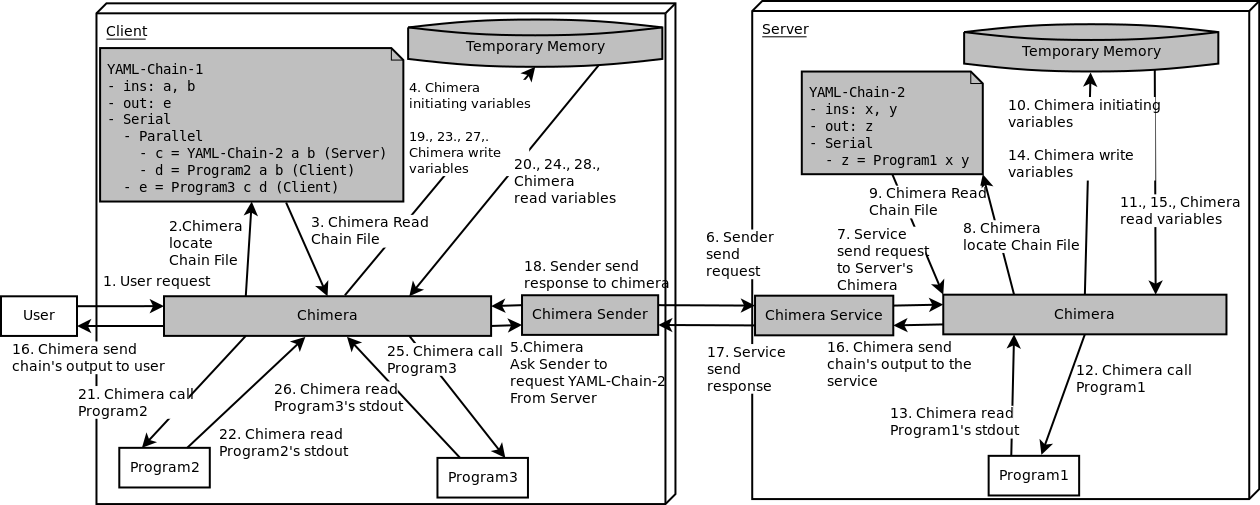
\includegraphics[width=1.0\textwidth]
		{images/chimera.png}
	\caption{Architecture of Chimera}
	\label{fig:chimeraArchitecture}
\end{figure*}

\section{Chimera Technical Implementation}

We already publish Chimera as NPM package. It is accessible through 
https://www.npmjs.com/package/chimera-framework.


\subsection{Node.js}

Node.js is a JavaScript runtime built on Chrome's V8 JavaScript engine. Node.js uses an event-driven, non-blocking I/O model that makes it lightweight and efficient \cite{nodejs}. Compared to Python and PHP, Node.js has an overall better performance
\cite{lei2014performance}.

Node.js has a package-manager named NPM (Node Package Manager). This allows developers
to use libraries that were already written by other developers. Chimera itself depend
on several packages:

\begin{itemize}
    \item async
    \item express
    \item fs-extra
    \item http
    \item js-yaml
    \item node-cmd
    \item path
    \item process
    \item querystring
\end{itemize}

\subsection{YAML Chain}
\blindtext

\subsection{JSON Formatted Temporary Global Storage}
\blindtext

\subsection{Parallel Processing}
\blindtext

\subsection{Web Service}
\blindtext


\section{Conclusion}
\blindtext 

%\appendices
%\section{Proof of the First Zonklar Equation}

% use section* for acknowledgement
\section*{Acknowledgment}
The authors would like to thank...

% Can use something like this to put references on a page
% by themselves when using endfloat and the captionsoff option.
\ifCLASSOPTIONcaptionsoff
  \newpage
\fi

\bibliographystyle{IEEEtran}
\bibliography{./citation}

% that's all folks
\end{document}

